\chapter{Attacks on privacy} \label{section: MIA}
\section{Membership inference attacks}
An attack model that plays a big role in machine learning is a membership inference attack.
With this attack, an adversary attempts to infer the original data point $x \in X$ from a given data point $z \in Z$.
The adversary has access to a point $z$, the size of the dataset $|Z|$ and a distribution D where $Z$ was drawn from \citep{yeom_privacy_2018}.
These attacks depend on the adversarial knowledge, which can be divided into white-box and black-box MIA's \citep{hu_membership_2022}.
\begin{enumerate}
  \item \textbf{White-box}: The attacker has all the data that is needed. Including target model parameters, the training dataset and even the architecture \citep{hu_membership_2022}.
  \item \textbf{Black-box}: The attacker has a limited amount of information, like training data distribution and the trained model \citep{hu_membership_2022}.
\end{enumerate}

An approach called \textit{Binary classifier membership inference attacks} is used to separate members from non-members. \citep{hu_membership_2022}.
This method evolves around the attacker generating a shadow model, with as goal to overfit \citep{shokri_membership_2017}.
If the data is fed with real data the score is higher than similar data, which means the real data can be inferred \citep{shokri_membership_2017,jayaraman_evaluating_nodate}
A white-box setting requires a lot of adversarial knowledge for training the shadow models.
The black-box settings only take the prediction as input and decide if it is a (non-) member \citep{hu_membership_2022}.
An unsupervised black-box MIA was introduced by Peng et al. and only considers that the attacker has access to the already trained model.
They rescale the probabilities first using temperature scaling, to compensate for models that are overconfident \citep{peng_unsupervised_nodate}.
So instead of having a probability between two classes with for example 99\% against 1\% it will be more evenly distributed based on the training data.
They then proceed in clustering the probabilities into two clusters using K-Means and label the higher confidence scores as members.

The above attacks do rely on the model to also provide the confidence or probabilities of the predictions.
This is often not the case for the practical appliance of a model, and therefore Choquette-Choo et al. introduced a label-only attack.
While the existing models exploit the probability output for MIA, they solely rely on labels.
For this, they make use of the "HopSkipJump" attack; a so-called decision-based attack \citep{chen_hopskipjumpattack_2020}.
Choquette-Choo et al. consider a more semi-black-box approach, for which the attacker still requires access to a subset of the original training data and the trained model.
Another paper that also uses "HopSkipJump" requires only the trained model and achieves higher accuracy by using an approach with random data \citep{li_membership_2021}.

Another take on this is prediction and confidence-based MIA which are both proposed by \citep{yeom_privacy_2018}.
They assume that an attacker knows the standard error and has access to the perturbation dataset.
The algorithm is then able to extract the truth label by minimizing the loss. \newline

\todo[inline]{Write summary / conclusion}
%To conclude on this, there are many methods for MIA and in that regard, the black-box approaches look the most promising.
%They require less setup and there is plenty of black-box approaches score with a success rate of 70\% and 80\%.
%For our use case, however, it is harder to establish an MIA; as we focus mainly on clustering.
%Anyhow, it is possible if we consider a semi-supervised approach where we consider the cluster labels as ground truth.
%%Differential privacy is proposed as a wmay of solving the inference attack for both white-box and black-box \citep{hu_membership_2022}.
%%However, it is hard to find a way to protect privacy and utility as well, so it depends heavily on the privacy budget.
\todo{Describe how dp is used to protect MIA}
\newpage
\section{Reconstruction attack}
This attack is a threat, especially to differential privacy.
The attack is primarily focused on reconstructing the data rather than focusing on machine learning.

% \section{Poison attack}
%\textbf{Reconstruction attacks:}
%Another attack that is a threat, especially to differential privacy is a reconstruction attack.
%This attack is also more known as the attribute inference attack and is more focused on the data itself than machine learning models \citep{rigaki_survey_2021}. 

%\textbf{Model extraction attacks:}
%The final attack that is considered, is the model extraction attack.
%This attack consists of the attacker being able to reconstruct and gather information about the original model.

% Jayaraman et al. evaluate inference attacks and differential privacy and express a metric called "privacy leakage"  \citep{jayaraman_evaluating_nodate}.


\begin{figure}
  \label{fig:unsupervised-mia-attack}
  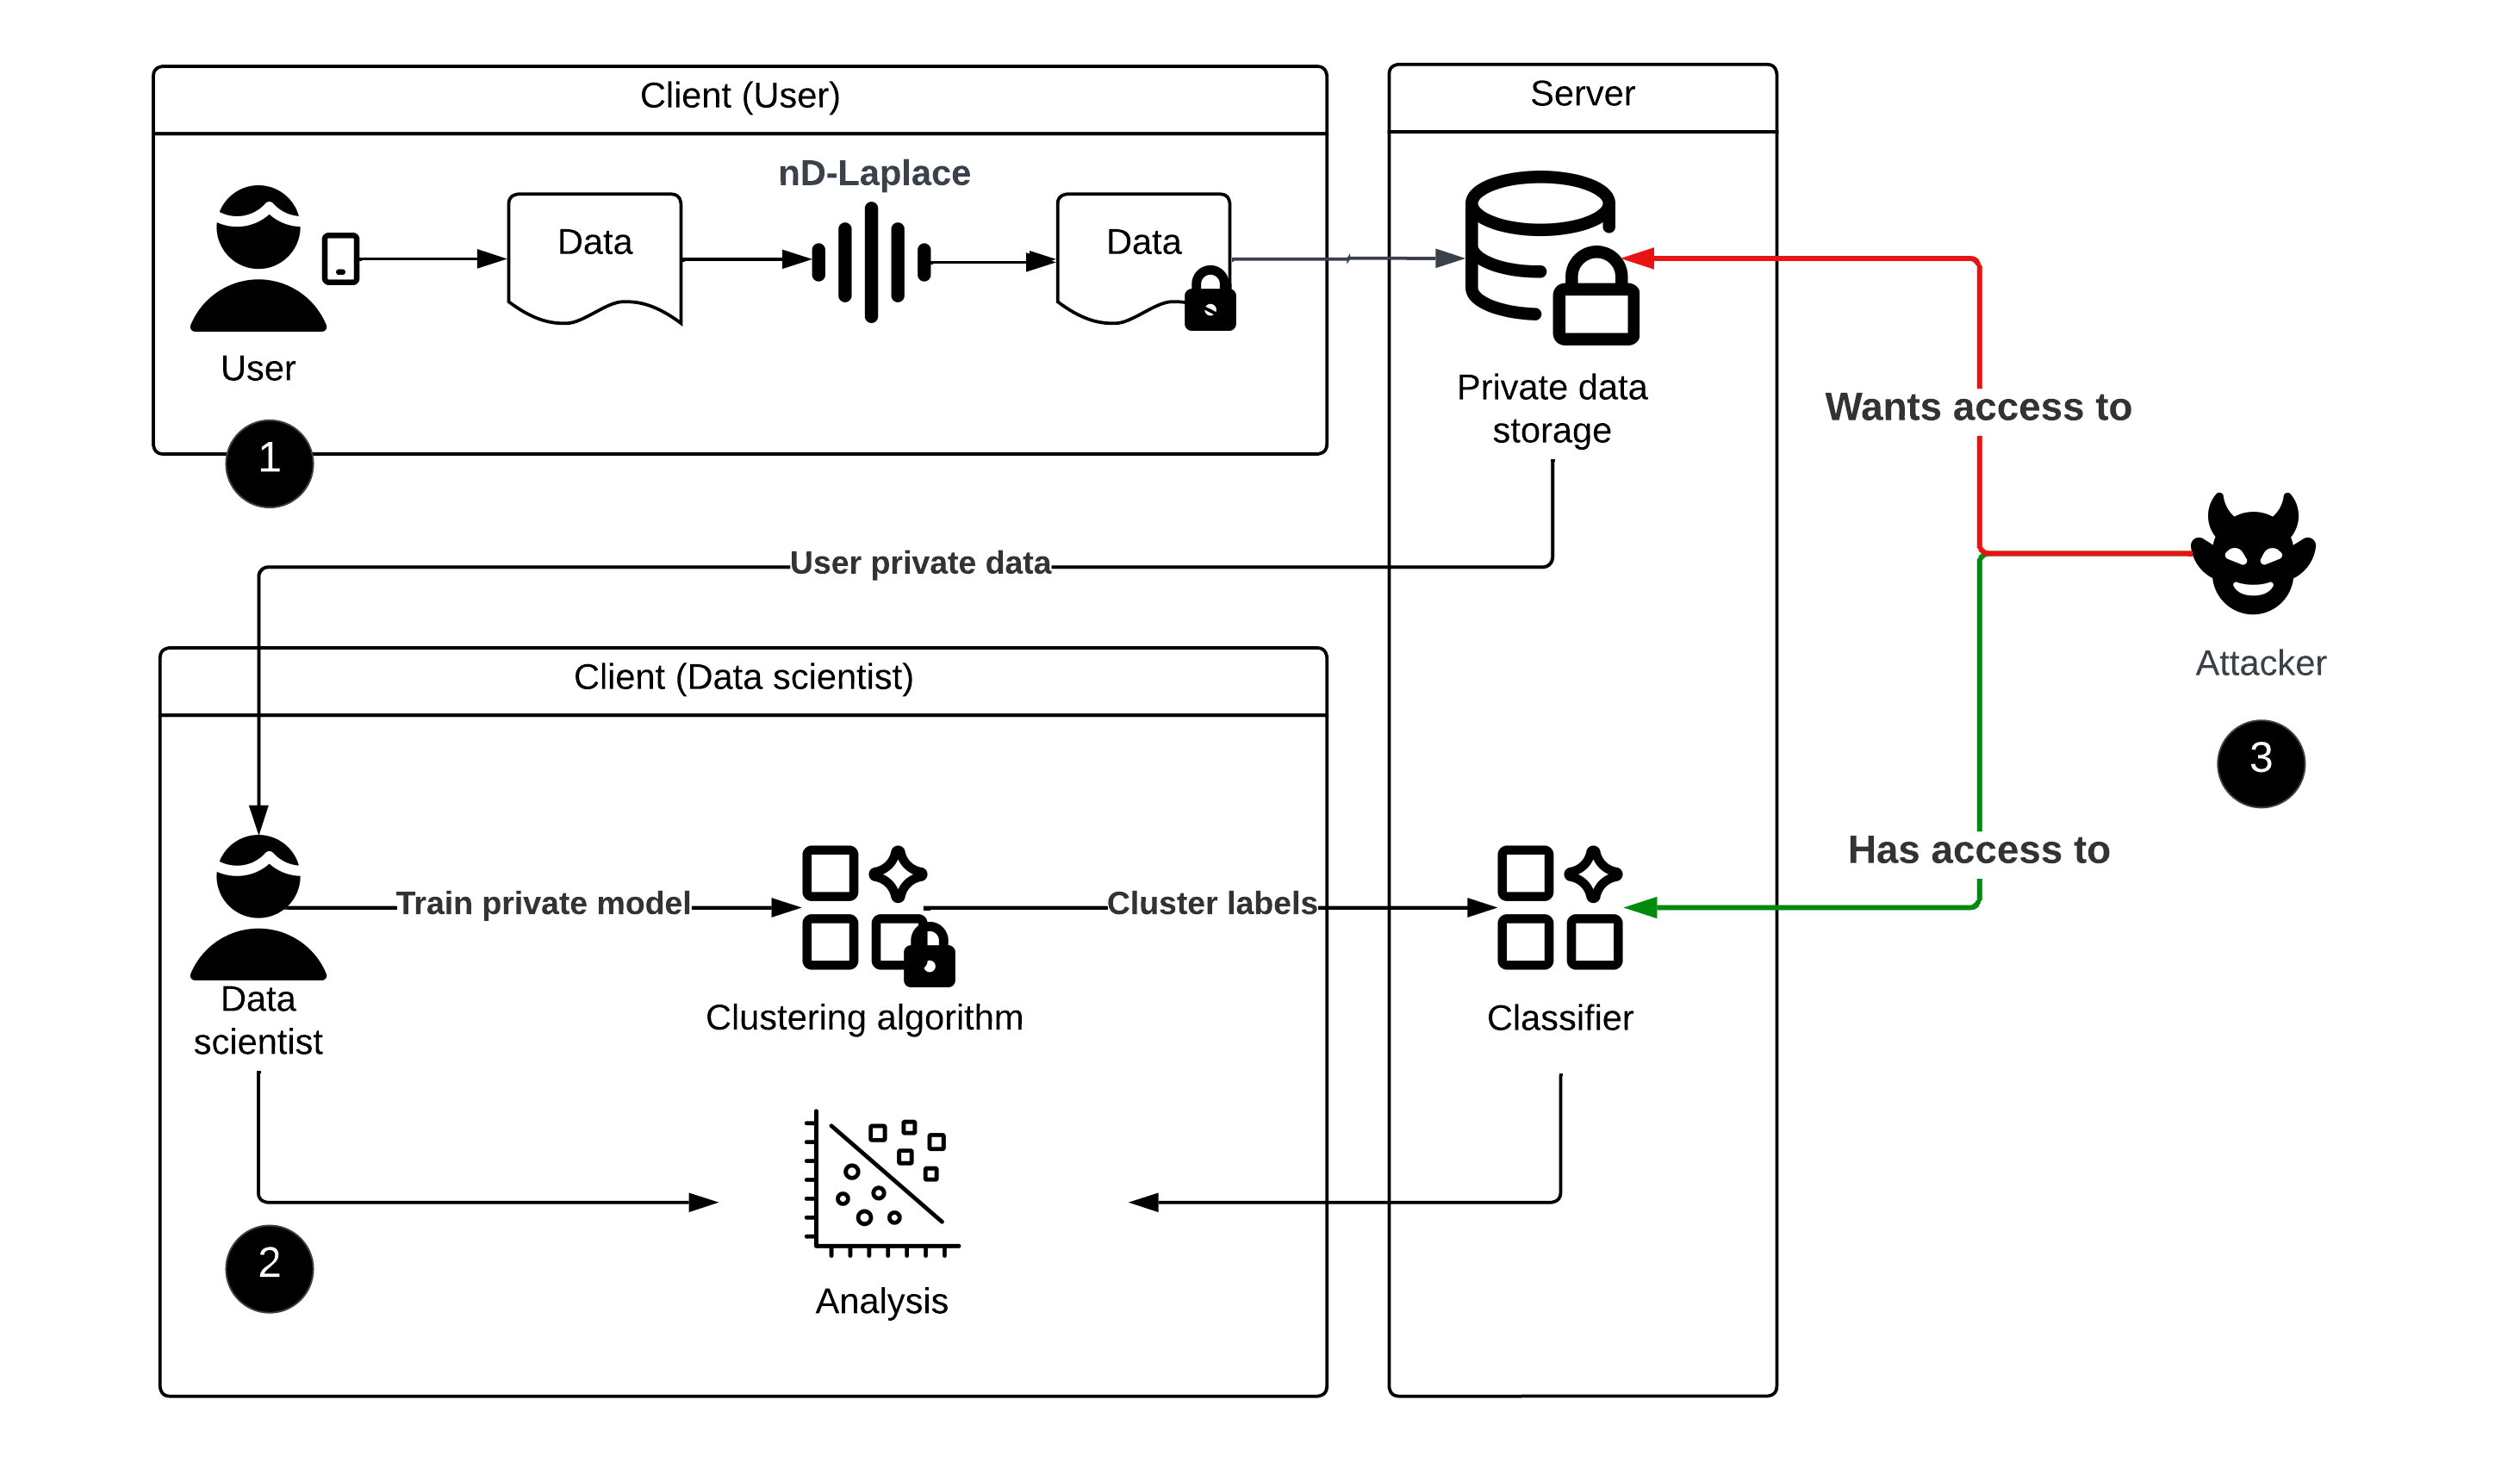
\includegraphics[width=1.0\textwidth]{TheorethicalFramework/Differential privacy/master-thesis-MIA.png}
  \caption{Semi-supervised membership inference attack considering a black-box approach \citep{chen_hopskipjumpattack_2020,li_membership_2021}}
\end{figure}
